% =====================================================================
%  c04 —— PDF p.34–38（原书 p.28–32）及原书 p.33 顶端
%  §2.2 二次微分形式与带状图（续）；§2.3 具有有限模的 Riemann 面上的两个不等式
% =====================================================================

% ===== 原书 p.28 =====
此时，把$E_{i,j}\subset\overline{D}_i$定义为
\[
E_{i,j}=\Bigl\{z_i\Bigm||z_i|=1,\ \sum_{p=1}^{j-1}s_{i,p}<\frac{s_i\arg(z_i)}{2\pi i}<\sum_{p=1}^{j}s_{i,p}\Bigr\},
\]
并使用变量
\[
w_{i,j}=\frac{s_i}{2\pi i}\log(z_i)+\sum_{p=1}^{j-1}s_{i,p}.
\]
同样定义$E_{i',j'}$、$w_{i',j'}$，并由$w_{i,j}+w_{i',j'}=0$把$E_{i,j}$与$E_{i',j'}$等同。
沿图$K$粘合诸$\overline{D}_i^*$。在$\partial E_{i,j}$处也把与图顶点对应之处等同。

\begin{center}
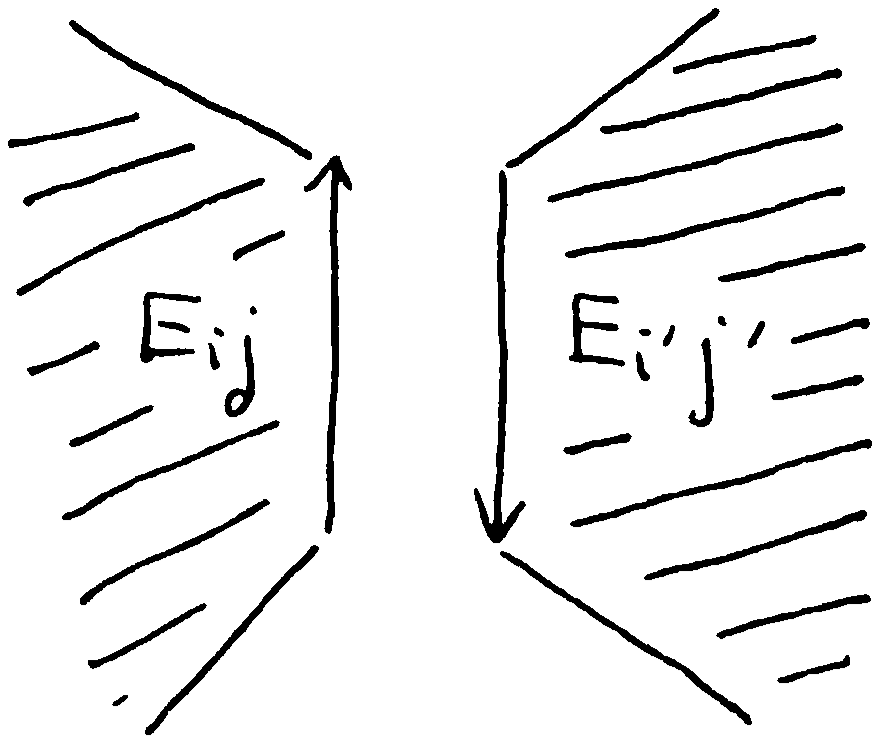
\includegraphics[width=0.40\linewidth]{fig_p34_a.png}
\end{center}

按照其顶点$v$处的价，即$\operatorname{val}(v)=\#\{e\mid v$是$e$的端点$\}$，用变量
\[
(*)\qquad u_v=w_{ij}^{\frac{2}{\overline{\operatorname{val}}(v)}}\exp\left(\frac{2\pi j\sqrt{-1}}{\operatorname{val}(v)}\right)
\]
来粘合。由此构成 r-punctured Riemann 面$(X,p_1,\dots,p_n)$。
在$\overline{D}_i^*$上用二次微分$\frac{r_i}{z_i^2}dz_i^{\otimes2}$来定义$\omega$，其中$r_i=\left(\frac{s_i}{2\pi}\right)^2$。
这一粘合得到$X$上在$p_1,\dots,p_r$有极点的二次微分，这可由
$dw_i=\frac{s_i}{2\pi i}\frac{dz_i}{z_i}$、$-dw_i^{\otimes2}=\frac{r_i}{z_i^2}dz^{\otimes2}$得知。
用坐标$u_i$在顶点$v$处表示$\omega$时，由关系$(*)$得
\[
dw^{\otimes2}=\left(\frac{\operatorname{val}(v)}{2}\right)^2u_i^{\operatorname{val}(v)-2}du_i^{\otimes2},
\]
故$\operatorname{ord}(\omega)=\operatorname{val}(v-2)$。又$\omega$在$p_i$处展开的$z_i^{-2}$的系数与$r_i$一致。
这样便构成了 Riemann 面$X$、$n$个点$p_1,\dots,p_n$及其上的二次微分$\omega$，它们满足定理 2.1 的条件。

\transnote{原文此处把点数一写作$n$、一写作$r$（「r-punctured 面$(X,p_1,\dots,p_n)$」之后紧接「$p_1,\dots,p_r$」）；照原文排印。}

\transnote{式$(*)$分母的$\operatorname{val}(v)$上多出一道上划线；照原文排印。}

\transnote{原文把$\operatorname{ord}(\omega)$印作$\operatorname{val}(v-2)$（应为$\operatorname{val}(v)-2$）；照原文排印。}

\subsection{具有有限模的 Riemann 面上的两个不等式}

Riemann 面上的有界开集$R$若含有与$R$同伦等价的$S^1$，则称之为环域。
（此处「有界」指不与$\C-\{0\}$
% ===== 原书 p.29 =====
全纯等价。）此时可知，存在唯一的$r\ge0$，使$R$与$\C$的区域$R_r=\{z\in\C\mid r<|z|<1\}$全纯等价。
$R$的模$M$由$M=-\frac{1}{2\pi}\log r$定义。此时$0<M\le\infty$。
换一种说法，$M$就是使$R_r-\R_{>0}$在$\frac{1}{2\pi i}\log(z)$下的像为
$\{x+yi\mid0<x<1,\ 0<y<M\}$的那个数。

\begin{center}
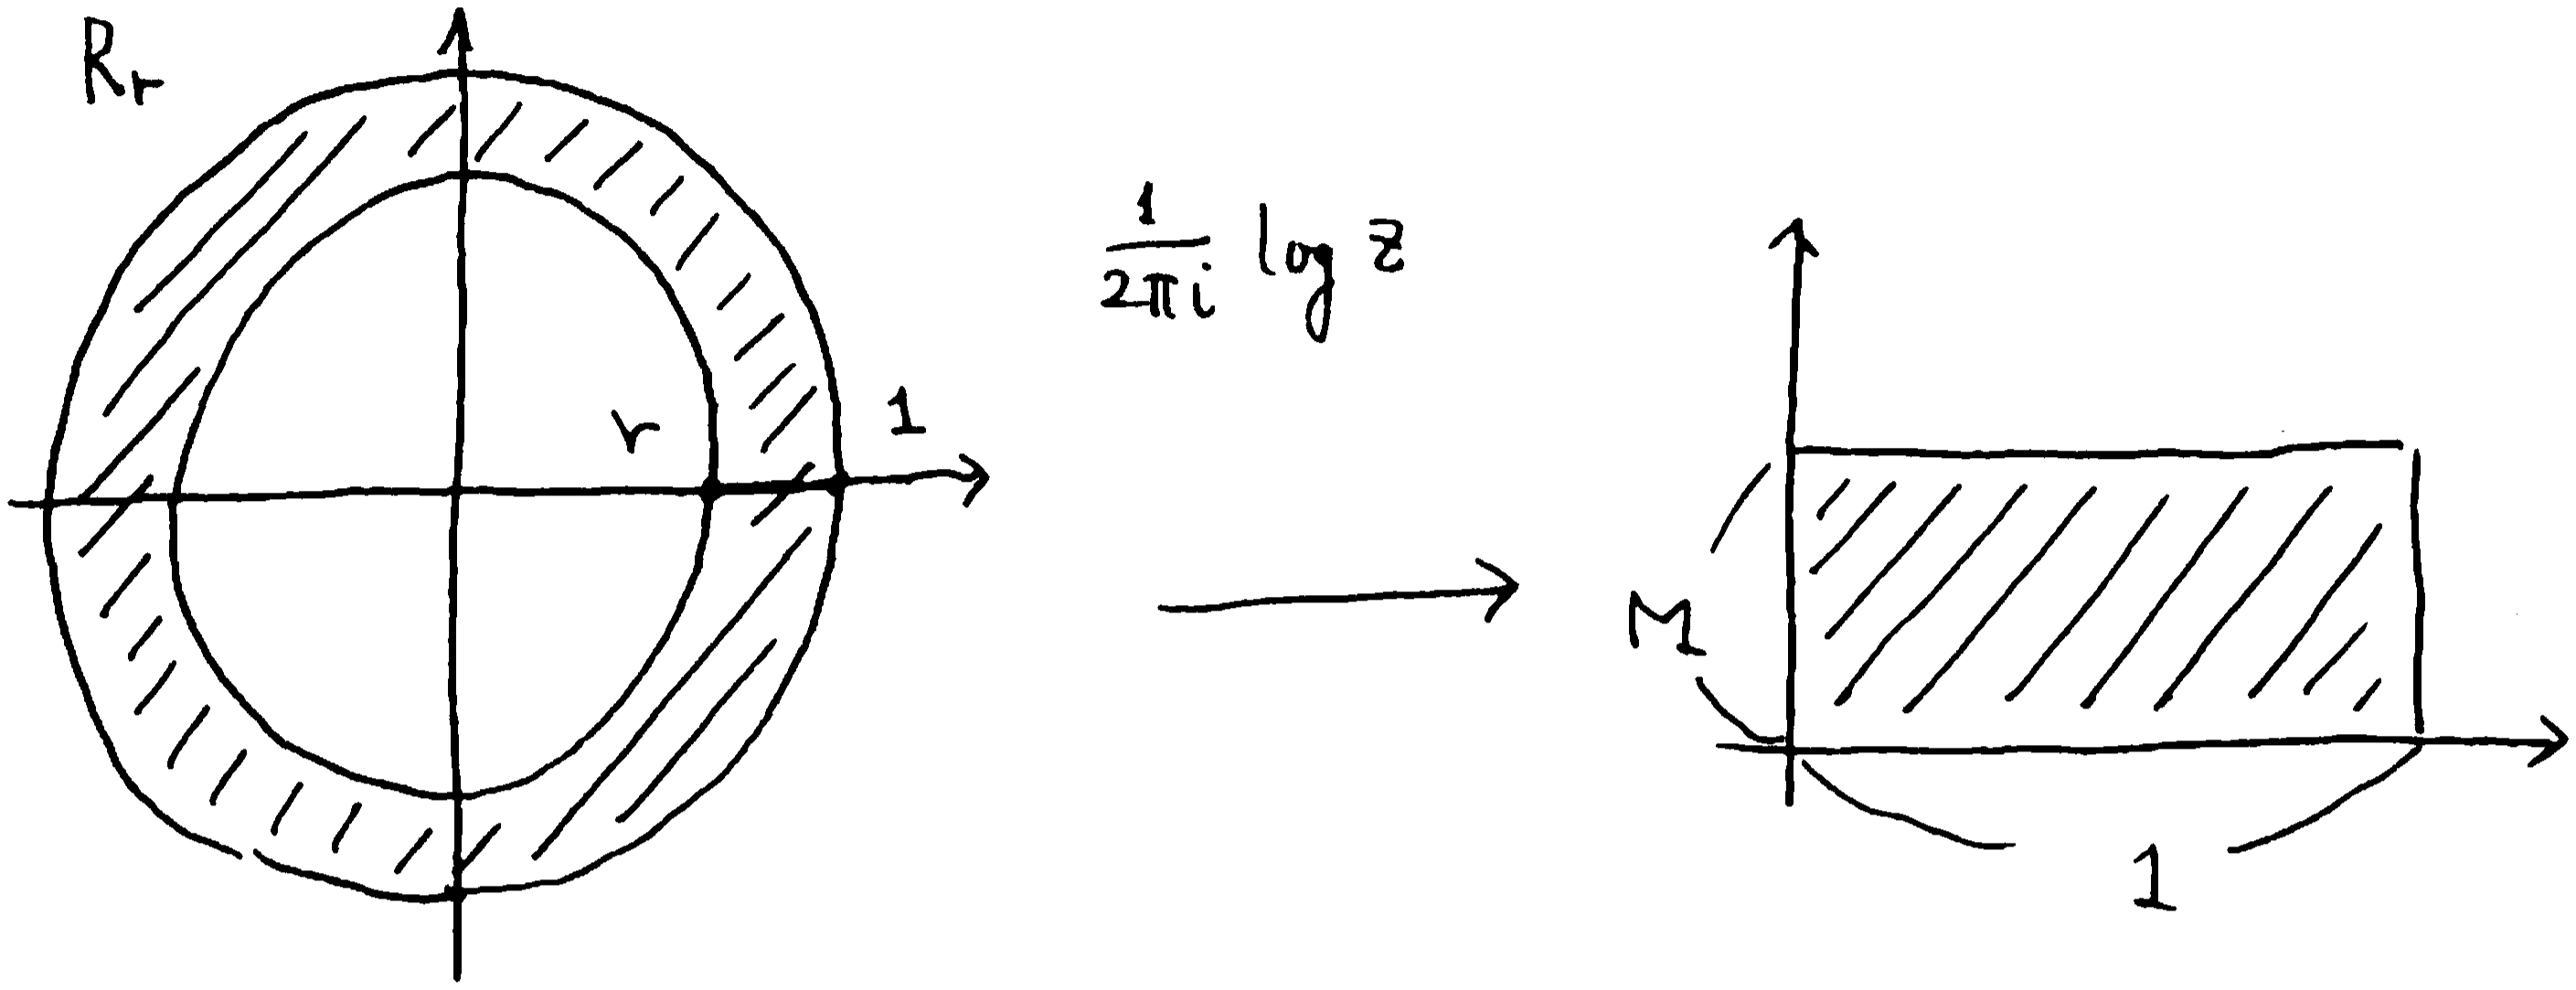
\includegraphics[width=0.88\linewidth]{fig_p35_a.png}
\end{center}

现设两个环域$R^{(1)},R^{(2)}$为有限模，且$R^{(1)}\subset R^{(2)}$，则$R^{(2)}$的模不小于$R^{(1)}$的模；
若两者一致，则$R^{(1)}=R^{(2)}$。在这个意义上，模衡量着环域的「大小」。
$D^*=\{z\mid0<|z|<1\}$的模为$\infty$，这种情形下有时也希望有计量「大小」的指标。
此时缩减模的概念就有用。设$t$为$D^*$在原点处的单值化参数。
定义$(D^*,t)$的缩减模为$\frac{1}{2\pi}\log\left|\frac{dt}{dz}(0)\right|$。
一般地，设区域$R\subset X$与$D=\{z\mid|z|<1\}$全纯等价，$p$为$R$上一点，$t$为$p$处的单值化参数。
此时$(R,p,t)$的缩减模定义为：取$\psi\colon R\xrightarrow{\ \sim\ }D$使$\psi(p)=0$，
再取$(D^*,\psi^{-1}(t))$的缩减模。
现设$R^{(1)}\subset R^{(2)}$与$D$全纯等价，$p\in R^{(1)}$，$t$为$p$处的单值化参数。
设$(R^{(i)},p,t)$的缩减模为$M_i$（$i=1,2$），则$M_1\le M_2$，等号仅在$R^{(1)}=R^{(2)}$时成立。
这样，此时也借助单值化参数$t$计量了环域的大小。

考察环域$R_r=\{z\mid r<|z|<1\}$及其上的二次微分$\omega=\frac{a^2}{z^2}dz^{\otimes2}$，
则按上节定义的$\psi(z)=\int\sqrt{\omega}$，$R_r-\R_{>0}$的像可表为
$\{x+yi\mid0<x<a,\ 0<y<aM\}$，故其面积表为$a^2M$。
这里要注意，$a$是与$R_r$同伦等价的轨道的长度。

% ===== 原书 p.30 =====
给定$X$上的二次微分$\omega$以及与$S^1$同胚的$\omega$的轨道$\gamma$（以下称之为闭轨道）时，
可知
\[
R_r=\{\gamma':\text{闭轨道}\mid\gamma'\text{与}\gamma\text{同伦}\}
\]
仍是环域。称之为$(\omega,\gamma)$对应的特征环域。
设$R_\gamma$为$(\omega,\gamma)$对应的特征环域，则与$\gamma$同伦的闭轨道$\gamma'$的长度
$a_{\gamma'}$等于$\gamma$的长度$a_\gamma$。称之为$R_\gamma$的长度。
设$R_\gamma$的模为$M_\gamma$，称$b_\gamma=a_\gamma M_\gamma$为$R_\gamma$的高。
由前面的计算，用$\omega$量出的$R_\gamma$的面积为$a_\gamma^2M_\gamma$。
若有有限个闭轨道$\gamma_1,\dots,\gamma_n$使$X-\bigcup_{i=1}^nR_{\gamma_i}$为测度$0$集，
则称$\omega$具闭轨道。此时称$(\gamma_i)_i$为闭轨道的型。
若$\omega$具闭轨道，则$X$的面积表为
\[
\|\omega\|_X=\sum_{i=1}^n a_{\gamma_i}^2M_{\gamma_i}.
\]

\transnote{原文此处的显示式印作$R_r$，而紧接的正文用$R_\gamma$；此处照原文排印。}

\begin{definition}[容许曲线系]
$X$内的简单闭曲线$\gamma_1,\dots,\gamma_n$称为容许的，指它们互不同伦，且不相交。
\end{definition}

\begin{lemma}
设$\omega$为 Riemann 面$X$上的二次微分，$\gamma_1,\dots,\gamma_n$为$X$上的容许曲线系。
设$R_i\subset X$（$i=1,\dots,n$）为互不相交且与$\gamma_i$同伦的环域。
设与$\gamma$同伦的$S^1$用$\omega$量出的长度的最小值为$a_i$，$R_i$的模为$M_i$，则
\[
\sum a_i^2M_i\le\|\omega\|_X.
\]
此外，若$\omega$具型$(\gamma_i)_i$的闭轨道，则上式中等号成立时，$R_i$与$\gamma_i$的特征环域$R_i$一致。
\end{lemma}

\transnote{原文此句用裸的$\gamma$（其余各处作$\gamma_i$），且最后一句把特征环域记作$R_i$，按文意应为$R_{\gamma_i}$；均照原文排印。}

\begin{proof}
令$r_i=\exp(-2\pi M_i)$。设$\varphi$为给出$R_i\subset X$与$R_{r_i}$全纯等价的映射，
再设它经$\frac{a_i}{2\pi i}\log\varphi(z)$把$R_{r_i}-\R_{>0}$映入长方形$S_i$，
则在此映射下由$\omega$决定的度量为$\rho(x,y)\sqrt{dx^2+dy^2}$。
又该长方形的高可用模$M_i$写成$b_i=a_iM_i$。现对$0<\mu<b_i$的$\mu$，
% ===== 原书 p.31 =====
$S_i$内的直线$(\R+\mu\sqrt{-1})\cap S_i$用$\rho(x,y)\sqrt{dx^2+dy^2}$量出的长度不超过$a_i$。
\[
a_i\le\int_0^{a_i}\rho(x+iy)dx\qquad(0\le y\le b_i)
\]
再对$y$从$0$到$b_i$积分，得
\[
a_ib_i\le\int_{S_i}\rho(x,y)dxdy.
\]
因此
\[
\sum_{i=1}^n a_ib_i\le\sum_{i=1}^n\int_{S_i}\rho(x,y)dxdy.
\]
用 Schwartz 不等式，
\begin{align*}
\left(\sum_{i=1}^n a_ib_i\right)^2
&\le\left(\sum_{i=1}^n\int_{S_i}\rho(x,y)dxdy\right)^2\\
&\le\left(\sum_{i=1}^n a_ib_i\right)
  \left(\sum_{i=1}^n\frac{1}{a_ib_i}\left(\int_{S_i}\rho(x,y)dxdy\right)^2\right)\\
&\le\left(\sum_{i=1}^n a_ib_i\right)
  \left(\sum_{i=1}^n\int_{S_i}\rho(x,y)^2dxdy\right).
\end{align*}
因$\int_{S_i}\rho(x,y)^2dxdy=\|\omega\|_{S_i}$，故
\[
\sum_{i=1}^n a_ib_i\le\sum_{i=1}^n\|\omega\|_{S_i}\le\|\omega\|_X.
\]

\transnote{原书把 Schwarz 拼作 Schwartz；照原文排印。}
后半部分的证明如下。若$\omega$具型$(\gamma_i)_i$的闭轨道，则$a_i$为$\gamma_i$的长度。
上面等号成立意味着向量$(\sqrt{a_i,b_i})_i$与
$\left(\frac{1}{\sqrt{a_ib_i}}\int_{S_i}\rho\,dxdy\right)_i$平行，且$\rho$为常函数。
由此可知，证明开头所定义的$\frac{a_i}{2\pi i}\log\varphi$
与由二次微分$\omega$决定的$\psi(z)=\int\sqrt{\omega}$只相差一个常数倍。
该常数为实数，这一点由叶状结构的样子可知。
因此，$R_i$与$\omega$对应的$\gamma_i$的特征环域一致。
\end{proof}

\transnote{原文把向量印作$(\sqrt{a_i,b_i})_i$，多出一个逗号（应为$\sqrt{a_ib_i}$）；照原文排印。}

现设$X$为紧 Riemann 面，$p_1,\dots,p_n$为其上的$n$个点，$\omega$为二次微分。
挖去$p_i$周围的小圆盘$D_i$所得的 Riemann 面$\tilde X=X-\bigcup_{i=1}^nD_i$上，
关于由$\omega$决定的度量的面积有限。
由此，对任意的闭曲线$\gamma_i\subset X$，$\{M_i\mid M_i$为与$\gamma$同伦等价的环域的模$\}$有界。

试就缩减模考虑引理 2.2。

% ===== 原书 p.32 =====
\begin{lemma}
设$X$为紧 Riemann 面，$p_1,\dots,p_n$为$X$上的$n$个点，$z_1,\dots,z_n$为$p_1,\dots,p_n$处的单值化参数。
设$\omega$为二次微分，它具以绕$p_1,\dots,p_n$的小闭曲线$\gamma_1,\dots,\gamma_n$为型的闭轨道。
现设存在以$p_i$为 puncture、互不相交的环域$R_i'$，设$M_i'$为其缩减模，则
\[
\sum_{i=1}^n a_i^2M_i'\le\sum_{i=1}^n a_i^2M_i.
\]
其中$M_i$为$\gamma_i$的特征环域关于$z_i$的缩减模，$a_i$为其长度。
又若等号成立，则$R_i=R_i'$。
\end{lemma}

\begin{proof}
首先设把$R_i'$移到$D^*=\{z\in\C\mid0<|z|<1\}$的全纯同构为$\varphi_i$。令
$D_i(\varepsilon)=\{z\in R_i'\mid|\varphi_i(z)|\le\varepsilon\}$，
$R_i'(\varepsilon)=R_i'-D_i(\varepsilon)$，$R_i(\varepsilon)=R_i-D_i(\varepsilon)$，
$X(\varepsilon)=X-\bigcup_{i=1}^nD_i(\varepsilon)$。
与引理 2.2 证明的前半部分相同，若$|\varphi_i(x)|=\mathrm{const}\ge\varepsilon$中存在非闭轨道者，
则存在$\delta>0$使
\[
\sum_{i=1}^n a_i^2M_i'(\varepsilon)+\delta\le\|\omega\|_{X(\varepsilon)}.
\]
两边加上$\sum_{i=1}^n\frac{a_i}{2\pi i}\log(\varepsilon)$，并令$\varepsilon\to0$。此时
\[
M_i'(\varepsilon)+\frac{1}{2\pi i}a_i^2\log(\varepsilon)=M_i',\qquad
\lim_{\varepsilon\to\infty}\left(M_i(\varepsilon)+\frac{a_i}{2\pi}\log(\varepsilon)\right)=M_i
\]
以及$\|\omega\|_{X(\varepsilon)}-\sum_{i=1}^nM_i(\varepsilon)\to0$，故得
\[
\sum_{i=1}^n a_i^2M_i'+\delta\le\sum_{i=1}^n a_i^2M_i.
\]
即使$|\varphi(z)|=\mathrm{const}$全为闭轨道，上面的不等式也以$\delta=0$成立。
又等号成立时，$\omega$在$X(\varepsilon)$上的限制为具闭轨道的二次微分，
故由引理的后半部分得$R_i(\varepsilon)=R_i'(\varepsilon)$。由此得$R_i=R_i'$。
\end{proof}

\transnote{原文此处印作$\lim_{\varepsilon\to\infty}$，按上下文应为$\varepsilon\to0$；照原文排印。}

迄今处理了关于长度与模的不等式，下面考察关于高与模的不等式。

\begin{theorem}
设$\omega$为具型$(\gamma_i)_i$的闭轨道、且$\|\omega\|_X<\infty$的二次微分。
设$R_i'$为互不相交的、与$\gamma_i$同伦等价的环域，
% ===== 原书 p.33 =====
% （本页只取定理 2.4 陈述的末段；证明由下一块承译。）
$M_i'$为其模，则
\[
\sum_{i=1}^n\frac{b_i}{M_i}\le\sum_{i=1}^n\frac{b_i}{M_i'}.
\]
其中$M_i$、$b_i$为$\gamma_i$对应的特征环域$R_i$的模与高。
又等号成立时，$R_i=R_i'$。
\end{theorem}
